\section{Experiment two}\label{sec:experiment_2}
This section will describe the second experiment of the project. The second experiment covers the necessary dimensions before reaching a threshold of 1\%, 5\%, and 10\% loss of accuracy. The experiment will only be done on 15.000 samples, instead of the entire data set of 60.000 samples, due to issues regarding memory usage. The experiment will focus on when different dimensionality reduction methods drop in accuracy due to too few dimensions and compare them to each other.


\subsection{Rules and evaluation of the experiment}\label{subsec:experiment_2_rules}
This section will cover the rules of the second experiment and how the experiment results will be evaluated.

The second experiment will be done on a subset of the entire data set. With 15.000 samples in the training set and the usual 10.000 samples in the test set. Instead of the standard 60.000 samples in the training set and 10.000 in the test set. The smaller sample size is used due to memory constraints regarding the non-linear methods, as they need more memory than was available.

The values from the mnist dataset will be normalized using standard scalar for each dimensionality reduction method. Ensuring the values are on the same scale so that different scales do not skew the results.

Hyperparameter tuning will be done using grid-search on each dimensionality reduction method. This is to ensure good hyperparameters are found for each number of components so that the results do not become skewed by hyperparameters that are not optimal for some parts of the model. If it was chosen to use a fixed value for the hyperparameters, the results could get skewed for a certain number of components.
The dimensionality reduction methods used are \gls{pca}, \gls{lda}, \gls{isomap}, and \gls{kpca}. The number of components will vary from around 2/5 to 50, and this range was chosen as it was believed to have a sufficient amount of components to show a general trend. For the non-linear methods, five components, instead of 2, were chosen as the lowest amount, as reducing the data to further takes much time, and the gain in insight was believed not to be worth the increased time cost. \gls{lda} is an exception, as the maximum number of components is the number of classes $-1$, which is 9 for the \gls{mnist}dataset, which means that the range of components for \gls{lda} will be from 2-9.

The values used to evaluate this experiment are \texttt{mean\_test\_score} based on \texttt{param\_pca\_\_n\_components} to evaluate the model's accuracy with the number of components used. Also, the \texttt{mean\_fit\_time} will be discussed as the time it takes to fit the model can determine how many components to use.

With the results from running the experiment, a plot shows the models' accuracy with the number of components used. The plot is used to represent when the accuracy starts to drop visually.

For each experiment, the data will be analyzed to see how many components can be removed before the accuracy drops below a certain threshold. For the experiment's sake, different thresholds will be used based on the highest value of accuracy for each of the methods. The thresholds will be a 1\% loss in accuracy, a 5\% loss in accuracy, and a 10\% loss in accuracy. These thresholds were chosen as they are believed to be a good balance between the number of components that can be removed and the amount of accuracy lost, which could be acceptable for some use cases.


\subsection{Results}\label{subsec:experiment_2_results}
This section will cover the results gathered from running the second experiment. Each of the dimensionality reduction methods will be presented using scatter plots. The scatter plots will show the number of components used along the x-axis and the model's accuracy along the y-axis. Each component has multiple dots, so the accuracy varies slightly depending on the hyperparameters used, but the general trend is the same. The results will then be compared and evaluated based on the experiment's rules. The main focus of the evaluation will be on when the accuracy starts to drop noticeably and how many components are needed to have good accuracy still. The scatter plots are used to represent the results visually, and the specific values of the accuracy will also be discussed. These values are taken from the csv\todo{add CSV to gls} files generated from running the second experiment.

\autoref{fig:experiment_2_pca_svm}.


\gls{pca} is a linear dimensionality reduction method; the scatter plot representing this method can be seen in \subsubsection{\gls{pca}}\label{subsubsec:experiment_2_pca}1.

As one would expect, the model's accuracy increases as the number of components increases. However, around 20 components, the accuracy starts to drop, the accuracy especially has a noticeable drop between 10 and 20 components, and the accuracy has a drastic drop for each component removed below ten components. This is expected as the lower the number of components the model has to work with; the more information is lost. With all 50 components, the model's accuracy is ~91.9\%, and first really drops below 91\% around 43 components.


\begin{figure}[htb!]
    \centering
    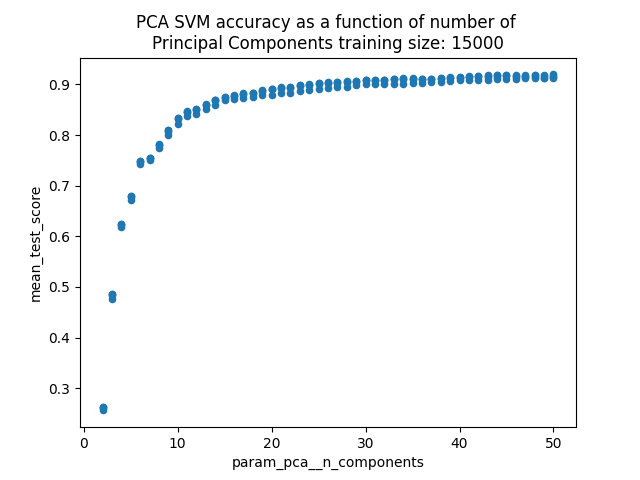
\includegraphics[width=0.8\textwidth]{figures/experiment_two/pca_svm_15000.png}
    \caption{Accuracy of the SVM model with \gls{pca} as dimensionality reduction method, with the number of components used.}
    \label{fig:experiment_2_pca_svm}
\end{figure}

For \gls{pca}, the highest accuracy value is 91.9\% with 50 components. The thresholds for \gls{pca} are: 91.9\% - 1\% = 90.9, 91.9\% - 5\% = 87.3\%, and 91.9\% - 10\% = 82.7\%. The results of the experiment for \gls{pca} will be compared to these thresholds.

By sorting the data by \texttt{mean\_test\_score} and going through the values, given the best-case scenario with the best hyperparameters found. The first value that drops below the threshold of 90.9\% is with an accuracy of 90.8\% at 31 components, which means that the model's accuracy only increases by 1\% with the last 19 components, which is close to half the total amount of components.
The next threshold of 87.3\% accuracy is found at 87.1\% with 16 components. By removing only three components, the accuracy dropped from a 1\% loss to a 5\% loss.
The final threshold of 82.7\% accuracy is found at 82.1\% with ten components. By removing only six components, the accuracy dropped from a 5\% loss to a 10\% loss.

\subsubsection{\gls{lda}}\label{subsubsec:experiment_2_lda}
\gls{lda} is another linear dimensionality reduction method, and the scatter plot representing this method can be seen in \autoref{fig:experiment_2_lda_svm}. \gls{lda} reduces the dimension to the number of classes $-1$, which is why the total number of components used is nine since \gls{mnist} has ten different numbers. The general trend is still valid for discussion in the second experiment.
Similar to \gls{pca}, the accuracy of the model increases as the number of components increases. However, around 6-7 components, a noticeable drop in accuracy can be seen. The highest accuracy score for \gls{lda} is 87.3\% with nine components, and the lowest accuracy score is 50.4\% with only two components. 

\begin{figure}[htb!]
    \centering
    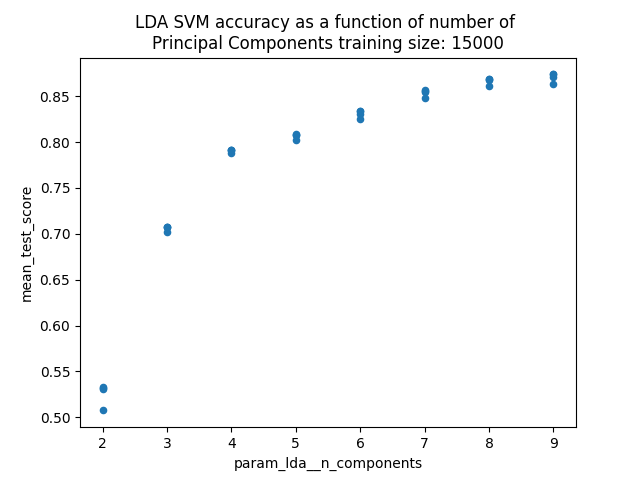
\includegraphics[width=0.8\textwidth]{figures/experiment_two/lda_svm_15000.png}
    \caption{Accuracy of the SVM model with \gls{lda} as dimensionality reduction method, with the number of components used.}
    \label{fig:experiment_2_lda_svm}
\end{figure}

For \gls{lda}, the highest accuracy score is at 87.3\% with nine components. The thresholds for \gls{lda} are: 87.3 - 1\% = 86.3\%, 87.3 - 5\% = 82.7\%, and 87.3 - 10\% = 78.1\%. The experiment's results for \gls{lda} will be compared to these thresholds.

Repeating the method of looking through the data gathered, the first value that drops below the first threshold of 86.3\% is at 86.2\% with all nine components. Some values with only eight components have a higher accuracy score, and some with a lower score than this—showing the impact of hyperparameter tuning.
The next threshold of 82.7\% accuracy is found at 82.4\% with six components. By removing three components, the accuracy dropped from a 1\% loss to a 5\% loss, which is not many components when compared to \gls{pca}, but for \gls{lda} that only has nine total components, a third of the components can be removed with a 5\% accuracy loss.
The final threshold of 78.1\% accuracy is found at 70.7\% with only three components. They are showing a significant drop from the threshold since the first few components impact the accuracy score significantly, and the closest value to the threshold is ~8\% away.


\subsubsection{\gls{kpca}}\label{subsubsec:experiment_2_kpca}
\gls{kpca} is a non-linear dimensionality reduction method, and the scatter plot representing this method can be seen in \autoref{fig:experiment_2_kpca_svm}.

\begin{figure}{htb!}
    \centering
    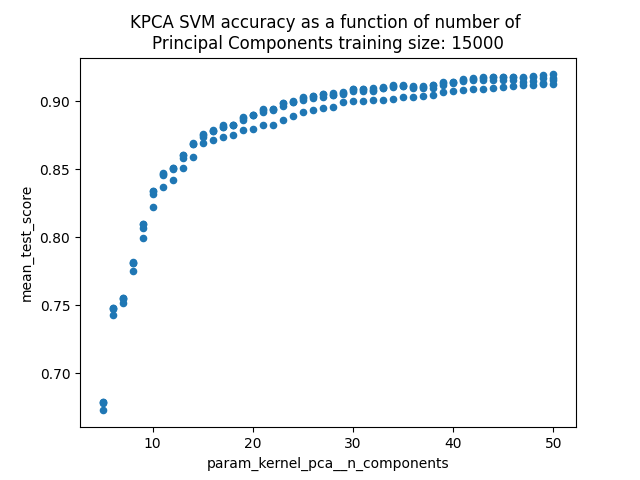
\includegraphics[width=0.8\textwidth]{figures/experiment_two/kpca_svm_15000.png}
    \caption{Accuracy of the SVM model with \gls{kpca} as dimensionality reduction method, with the number of components used.}
    \label{fig:experiment_2_kpca_svm}
\end{figure}

\autoref{fig:experiment_2_kpca_svm} is very similar to the other methods. However, it should be noted that although the accuracy seems to drop drastically as the number of components decreases, by comparing \autoref{fig:experiment_2_kpca_svm} and \autoref{fig:experiment_2_pca_svm}, it is seen that the accuracy of \gls{kpca} overall is higher than \gls{pca}. The highest accuracy score for \gls{kpca} is 91.9\% with 50 components similar to \gls{pca}, but the lowest accuracy score is 64.4\% with two components, unlike \gls{pca}, which has its lowest accuracy score of 25.6\%.

\gls{kpca} has a top accuracy score of 91.9\%, meaning that the thresholds for \gls{kpca} are: 91.9 - 1\% = 90.9\%, 91.9 - 5\% = 87.3\%, and 91.9 - 10\% = 82.7\%. The experiment's results for \gls{kpca} will be compared to these thresholds.

Similar to linear methods, the data is sorted by its accuracy score to find the first value where the accuracy drops below a threshold. The first threshold of 90.9\% accuracy is found at 90.8\% with 31 components. The next threshold of 87.3\% accuracy is found at 87.1\% with 16 components. The final threshold of 82.7\% accuracy is found at 82.1\% with ten components.


\subsubsection{\gls{isomap}}\label{subsubsec:experiment_2_isomap}
\gls{isomap} is the final method of the second experiment, which is non-linear, and the scatter plot representing this method can be seen in \autoref{fig:experiment_2_isomap_svm}.

\begin{figure}{htb!}
    \centering
    \includegraphics[width=0.8\textwidth]{example-image-a}
    \caption{Accuracy of the SVM model with \gls{isomap} as dimensionality reduction method, with the number of components used.}
    \label{fig:experiment_2_isomap_svm}
\end{figure}



\subsection{Discussion of experiment two}\label{subsec:experiment_2_discussion}
This section will discuss the results of the second experiment and compare the results of the different methods, first by discussing the results of the linear methods, then the non-linear methods, and finally, comparing the results of all methods.

For each section, a table will display the different percentages of components remaining before the accuracy drops below a threshold. The table will also show the number of remaining components to show the difference between the methods.


\subsubsection{Linear methods}
By comparing the two linear methods used for the second experiment, it is essential to know that the number of components is very different between \gls{pca} \gls{lda}, which means that an exact comparison between the two methods is not always clear. Instead of using the number of components as a comparison, the percentage of remaining components will be used to try and make a fair comparison. A table showing the differences between the two methods can be seen in \autoref{tab:experiment_2_linear_methods_comparison}.

\begin{table}[htb!]
    \centering
    \begin{tabular}{|c|c|c|}
        \hline
        \textbf{Thresholds} & \textbf{PCA \% of 50 Components} & \textbf{LDA \% of 9 Components} \\ \hline
        \textbf{1\%} & \textbf{62\% (31)} & \textbf{100\% (9)} \\ \hline
        \textbf{5\%} & \textbf{32\% (16)} & \textbf{66\% (6)} \\ \hline
        \textbf{10\%} & \textbf{20\% (10)} & \textbf{33\% (3)} \\
        \hline
    \end{tabular}
    \caption{Percentage of the components remaining after the threshold is reached, with the corresponding number of components in paratheses.}
    \label{tab:experiment_2_linear_methods_comparison}
\end{table}

\autoref{tab:experiment_2_linear_methods_comparison} shows, for each linear method, the amount of components left after each of the thresholds is reached. So for \gls{pca}, 62\% of the total number of components remaining before reaching the first threshold of 1\%, whereas, for \gls{lda}, there is 100\%.

From \autoref{tab:experiment_2_linear_methods_comparison}, it can be seen that before reaching the first threshold of losing 1\% accuracy, \gls{pca} can cut off 38\% of its components, before reaching the threshold, while \gls{lda} can not afford to lose any components. It shows that for \gls{lda}, the number of components and the hyperparameters have a significant impact and that it is not as easy to cut off components as it is for \gls{pca} without losing accuracy.

By comparing the two linear methods, it can be concluded that \gls{lda} is more prone to losing accuracy when removing components than \gls{pca}. The accuracy loss is likely because \gls{lda} has so few components to work in the first place. It could be argued that the results are not entirely fair since \gls{pca} has so many more components, but scaling the values with percentage should show a general trend.


\subsubsection{Non-linear methods}

\subsubsection{Comparison of methods}



% intro
% presentation af de experimenter vi har valgt og hvorfor vi har valgt dem?
% experiment 1 exemple
%     detaljeret gennemgang af regler og evaluering
%     fremvisning af resultater
%     opsumering af resultater
%     diskussion af resultater og hvad der ellers var spændende evaluering af hvorfor det blev sådan.

%logarithmic regression
%Bar chart